
% !TeX root = ../book.tex
% !TeX spellcheck = fr_FR
% !TeX encoding = ISO-8859-1

\section{Bricoles deux et trois bandes}\label{sec:B15}

Ce sont deux bricoles diff�rentes mais bien utiles et si souvent
n�glig�es au profit d'un 1B qui laisse la 1 au milieu des deux autres
billes.

Figure 1 : On s'est emp�tr� � la petite bande en tentant de rentrer les
billes 2 et 3. Un petit 1B ne serait pas une mauvaise solution mais elle
impose de nouveau un r�tro 1B � suivre et laisse la 1 avec une prise de
dominante difficile. Tentez donc une bricole 2B comme dessin� bille en
t�te sans effet et viser pour toucher la 2�bande juste devant la 2. La 1
aura tendance � prendre la dominante en un seul coup. Si par malheur ce
n'est pas parfaitement r�ussi, la situation ne sera pas d�t�rior�e par
rapport � la situation pr�c�dente.

Figure 2 : La position de la 3 est telle que son rappel est tr�s
difficile voire impossible. Un 1B sur la 3 donne un r�sultat tr�s
al�atoire. On devrait jouer assez fort et la 3 reviendrait au coin
pendant que la 2 change de c�t�. Un 1B sur la 2 est sans doute le point
le plus facile mais il donne une position tr�s inconfortable. Serrez
donc en un coup. Si la 2 n'est pas trop �loign�e de la petite bande,
appliquez une bricole deux bandes par l'arri�re, mi-hauteur ou mi-haute,
assez grosse et bon effet bien dos�. Les billes se retrouvent dans le
chapeau au croisillon du cadre. Au deuxi�me coup, vous aurez l'embarras
du choix pour � tourner � le jeu.

Remarques :
\begin{itemize}
	\item Une prise fine am�ne la 1 entre la petite bande et la bissectrice.
	\item Une prise moyenne am�ne vers la bissectrice.
\end{itemize}

Une prise grosse am�ne aussi vers la bissectrice avec une tendance � la
d�passer mais attention : pas beaucoup. Pour ramener la 1 plus pr�s de
la grande bande, il conviendra de bricoler bille basse avec un bon effet
maximum, presque coup du r�tro... - Le point est plus facile lorsque la
3 est un peu plus pr�s de la petite bande que la grande...

Notez bien : quel que soit l'essai, la position suivante sera presque
toujours favorable au jeu constructif. Ceci est un point typique du jeu
de cadre. Il demande une petite habitude pour jauger de la grosseur de
bille et l'�vitement de la bosse (pas toujours d�favorable) de la 1 sur
la 2 apr�s 3 bandes...


\begin{figure}[htb]
	\centering
	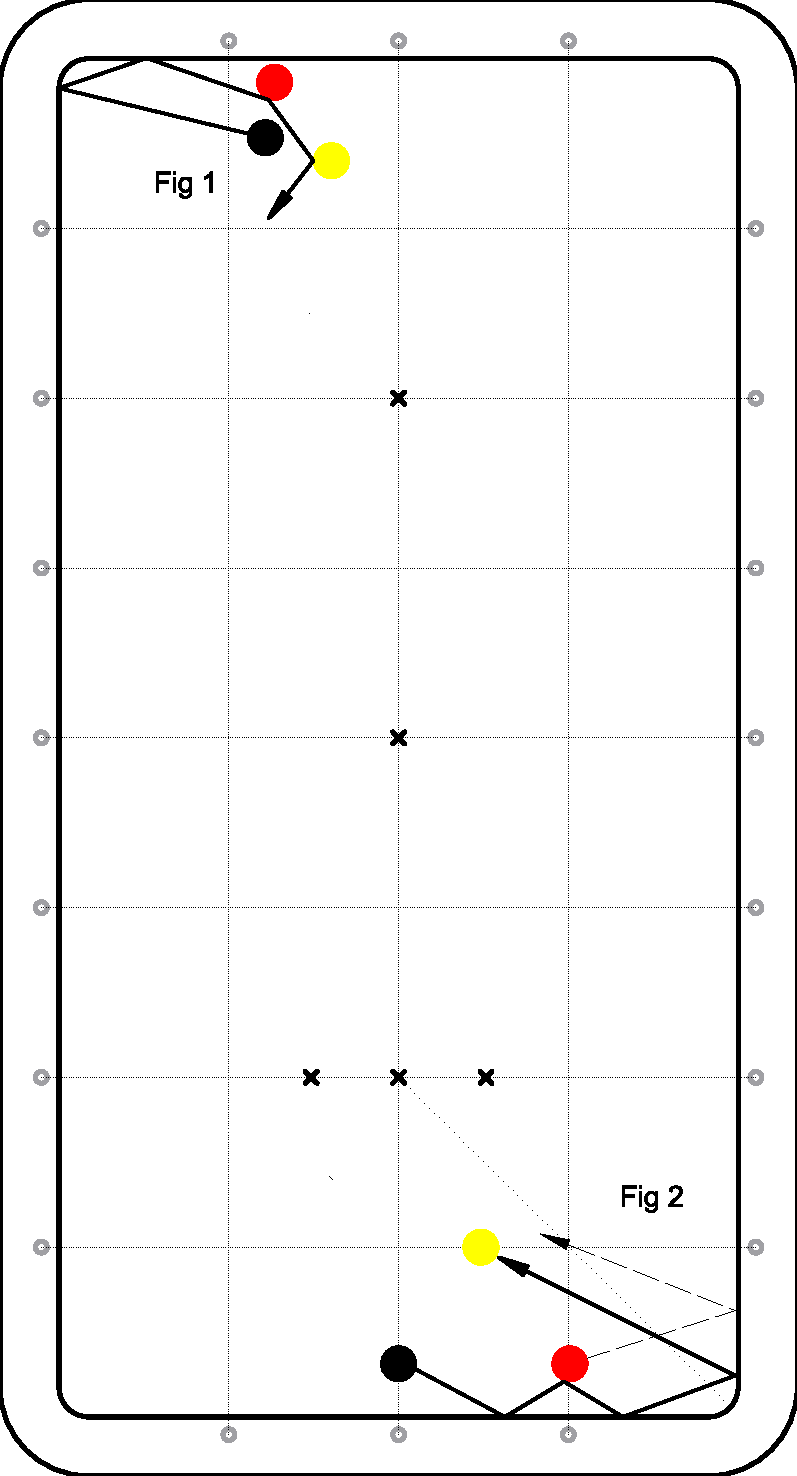
\includegraphics[width=0.85\linewidth]{B/imagesB/B15-01.pdf}
	\caption{Bricoles deux et trois bandes.}
	\label{fig:B15-1}
\end{figure}

\clearpage
